\documentclass[aspectratio=169]{beamer}
\usetheme{Madrid}
\usecolortheme{default}
\setbeamertemplate{footline}[frame number]

\usepackage{graphicx}
\usepackage{booktabs}
\usepackage{amsmath}
\usepackage{amssymb}
\usepackage{hyperref}
\usepackage{listings}
\usepackage{xcolor}

\title[IPS Veto Position Scan]{IPS Veto Position Scan for Deep Inelastic Event Tagging}
\subtitle{Geant4 study in the 3 deg, 1.15 T configuration}
\author{Tian Baiting}


\date{\today}

\lstset{
  basicstyle=\ttfamily\scriptsize,
  breaklines=true,
  frame=single,
  columns=fullflexible
}

\begin{document}

\begin{frame}
\titlepage
\end{frame}

\begin{frame}{Physics Goal}
\begin{itemize}
  \item The IPS detector is used as a veto counter for deep inelastic deuteron reactions.
  \item The optimization target is:
  \begin{itemize}
    \item maximize the IPS response to small-impact-parameter events,
    \item while suppressing the response to elastic deuteron breakup events.
  \end{itemize}
  \item The study reported here is the current \textbf{official full-statistics run}:
  \begin{itemize}
    \item geometry: \texttt{3deg\_1.15T},
    \item target: \texttt{reference only} (\texttt{Target/SetTarget false}),
    \item selection: \texttt{no-forward},
    \item signal proxy: all-event samples with $b_{\mathrm{imp}} \le 7$.
  \end{itemize}
\end{itemize}
\end{frame}



\begin{frame}{Detector and Coordinate Definition}
\begin{itemize}
  \item IPS is implemented as a 32-channel barrel in Geant4.
  \item Geometry parameters:
  \begin{itemize}
    \item 32 modules,
    \item module size: $20 \times 20 \times 200$ mm$^3$,
    \item barrel radius: 135 mm,
    \item angular pitch: $360 / 32 = 11.25^\circ$.
  \end{itemize}
  \item The target normal defines the local beam direction.
  \item The IPS barrel axis is parallel to this local beam direction.
  \item The scanned parameter is the signed axial displacement:
  \[
    \vec{r}_{\mathrm{IPS}} = \vec{r}_{\mathrm{target}} + s \, \hat{u}_{\mathrm{beam}},
  \]
  where $s$ is the \texttt{AxisOffset}.
\end{itemize}
\end{frame}

\begin{frame}{Proton px Scan at Offset 0 mm}
\begin{columns}[T]
\column{0.60\textwidth}
\centering
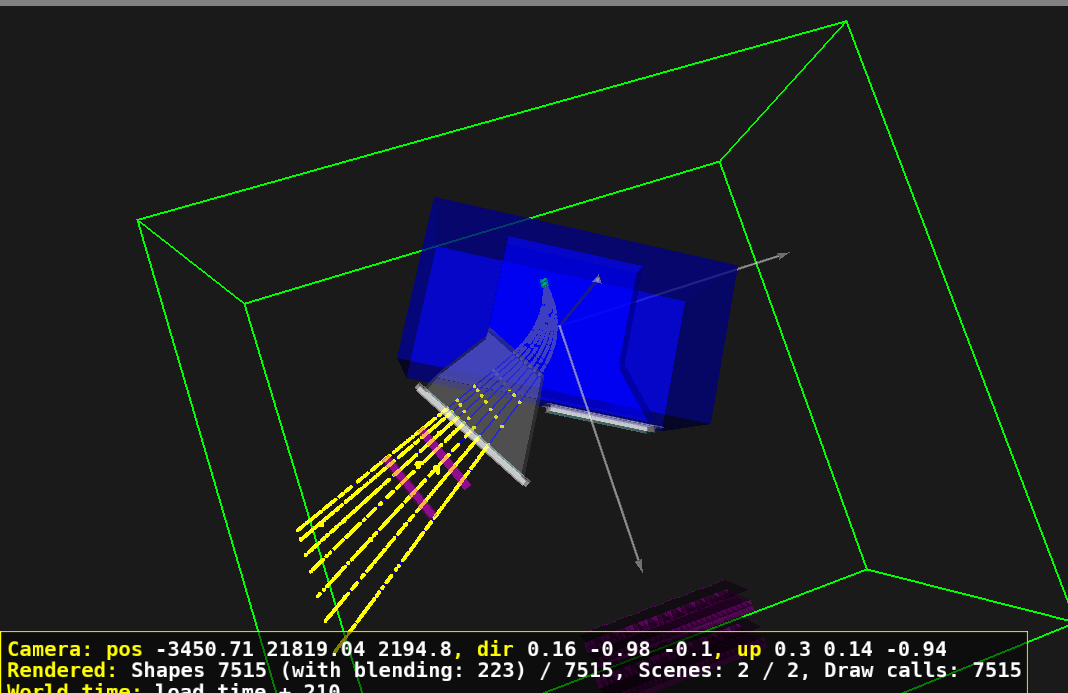
\includegraphics[width=\textwidth]{figures/2026-04-05-19-17-09.png}

\column{0.40\textwidth}
\small
\begin{itemize}
  \item One event contains 7 injected protons.
  \item Input family:
  \item \texttt{px = [+150, +100, +50, 0, -50, -100, -150] MeV/c}
  \item \texttt{py = 0 MeV/c,\ \ pz = 627 MeV/c}
  \item All tracks start from the same target-reference point.
  \item The apparent vertical spread in the rendered view comes from projection and magnetic bending, not from an initial $y$ dispersion.
\end{itemize}
\end{columns}
\end{frame}

\begin{frame}{Elastic Breakup Representative at Offset 0 mm}
\begin{columns}[T]
\column{0.58\textwidth}
\centering
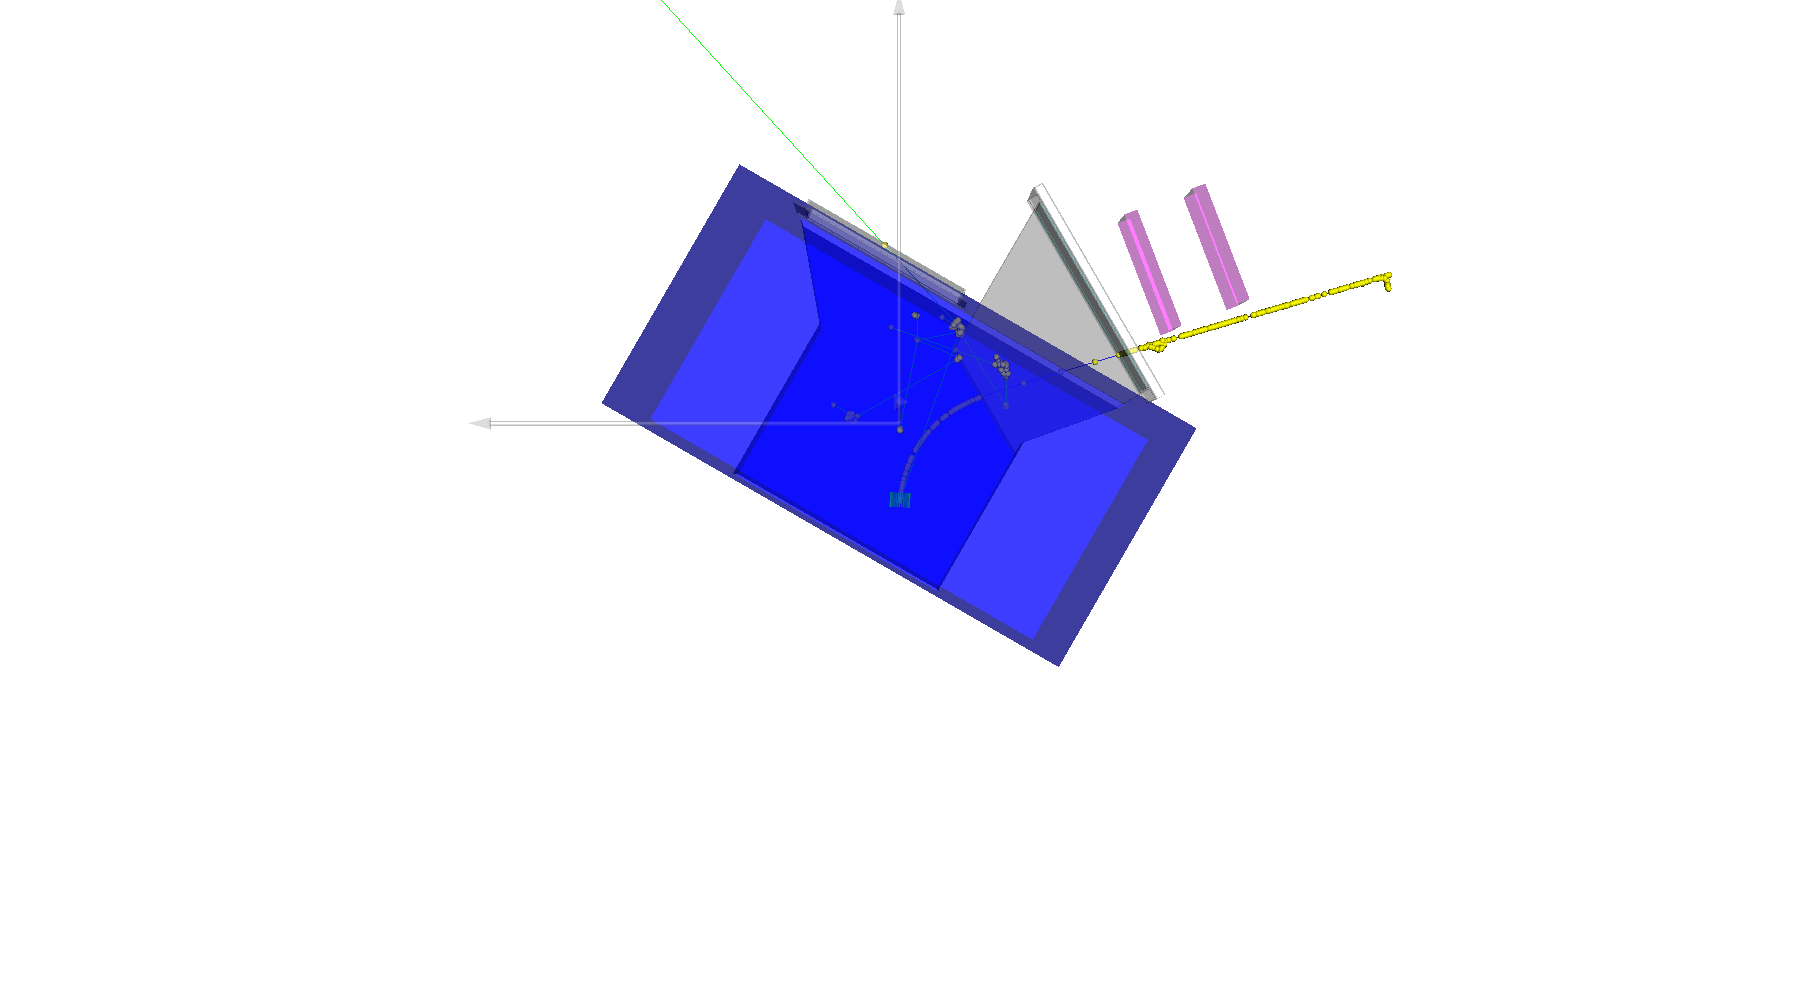
\includegraphics[width=\textwidth]{assets/ips_scan_3deg_1p15T_fullstats/event_visuals/elastic_b05_typical_offset0.png}

\column{0.42\textwidth}
\small
\begin{itemize}
  \item This picture uses the selected elastic representative from bucket \texttt{b05}.
  \item Event metadata:
  \begin{itemize}
    \item $b_{\mathrm{imp}} = 5$
    \item 2 final fragments
    \item 1 charged fragment
    \item IPS hit at 0 mm: no
  \end{itemize}
  \item Viewpoint: from $+y$ toward the $x$-$z$ plane.
  \item It is close to the median relative-momentum topology inside the cleaned elastic sample.
  \item These visual examples use \textbf{offset 0 mm} only for consistent illustration; the optimization itself is still performed over the full offset scan.
\end{itemize}
\end{columns}
\end{frame}

\begin{frame}{Small-b Representative Event at Offset 0 mm: Central Topology}
\begin{columns}[T]
\column{0.58\textwidth}
\centering
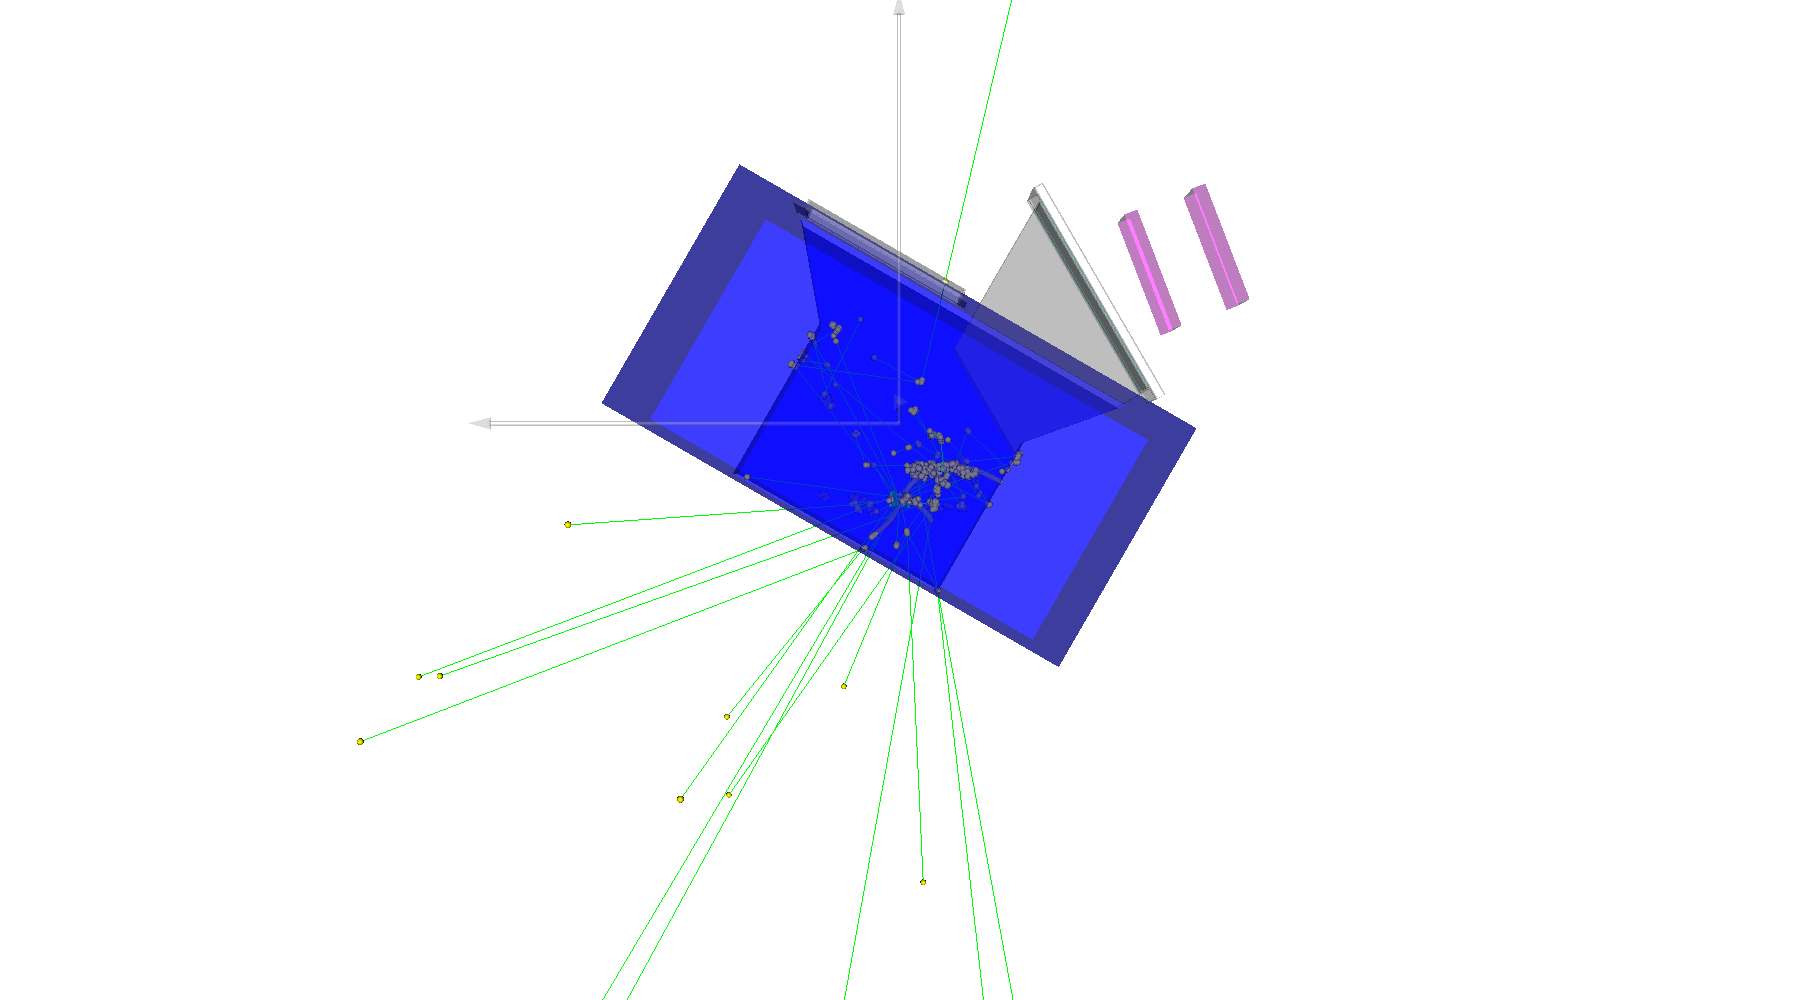
\includegraphics[width=\textwidth]{assets/ips_scan_3deg_1p15T_fullstats/event_visuals/allevent_b01_typical_offset0.png}

\column{0.42\textwidth}
\small
\begin{itemize}
  \item Representative all-event entry from bucket \texttt{b01}.
  \item Event metadata:
  \begin{itemize}
    \item $b_{\mathrm{imp}} = 1$
    \item 28 final fragments
    \item 6 charged fragments
    \item IPS hit at 0 mm: yes
  \end{itemize}
  \item Viewpoint: from $+y$ toward the $x$-$z$ plane.
  \item This is the kind of high-multiplicity central event that the veto should detect efficiently.
\end{itemize}
\end{columns}
\end{frame}

\begin{frame}{Small-b Representative Event at Offset 0 mm: Edge of the Signal Region}
\begin{columns}[T]
\column{0.58\textwidth}
\centering
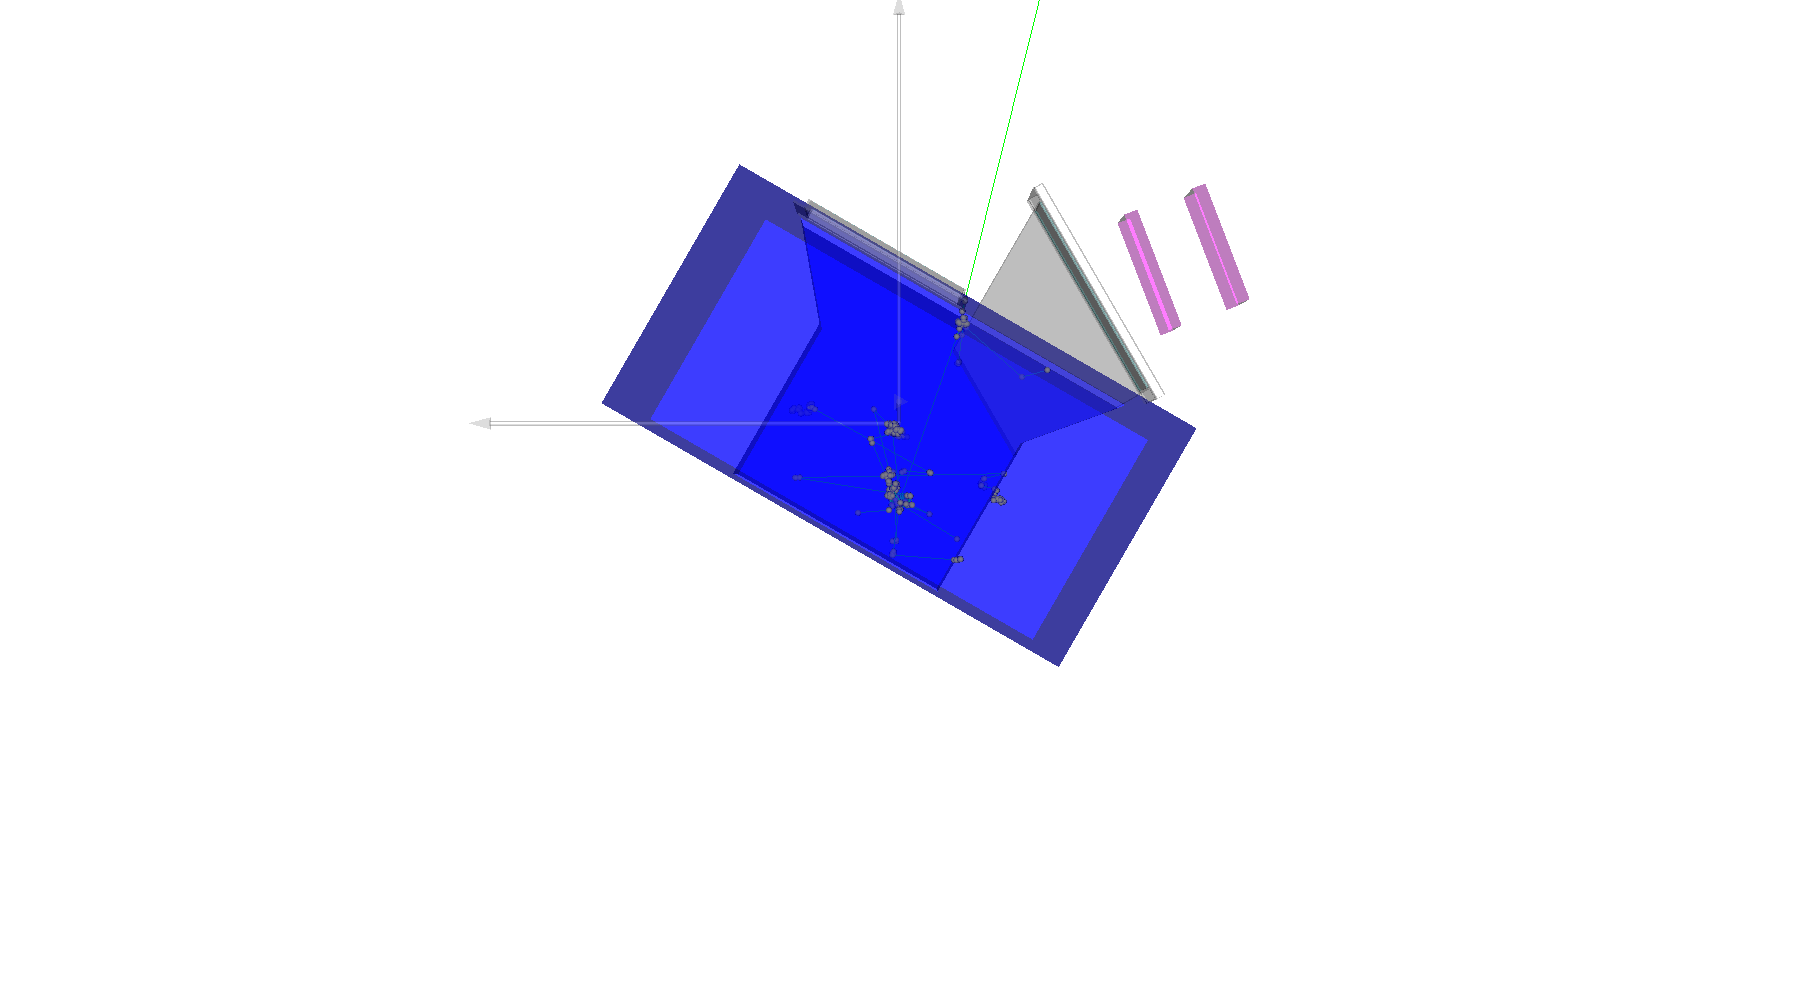
\includegraphics[width=\textwidth]{assets/ips_scan_3deg_1p15T_fullstats/event_visuals/allevent_b07_typical_offset0.png}

\column{0.42\textwidth}
\small
\begin{itemize}
  \item Representative all-event entry from bucket \texttt{b07}.
  \item Event metadata:
  \begin{itemize}
    \item $b_{\mathrm{imp}} = 7$
    \item 11 final fragments
    \item 2 charged fragments
    \item IPS hit at 0 mm: yes
  \end{itemize}
  \item Viewpoint: from $+y$ toward the $x$-$z$ plane.
  \item This event sits near the upper boundary of the small-$b$ signal definition and illustrates the lower-multiplicity end of the accepted topology family.
\end{itemize}
\end{columns}
\end{frame}

\begin{frame}[fragile]{Important Modeling Choice}
\begin{block}{Target is a reference point, not a material}
\begin{itemize}
  \item The primary particles already come from ImQMD post-reaction outputs.
  \item Therefore the target must \textbf{not} be inserted as a real material in Geant4.
  \item The run macros force:
\begin{lstlisting}
/samurai/geometry/Target/SetTarget false
/samurai/geometry/IPS/SetIPS true
/samurai/geometry/IPS/AxisOffset <offset> mm
\end{lstlisting}
  \item The target position and angle are still used to define the launch point and the IPS alignment axis.
\end{itemize}
\end{block}
\end{frame}

\begin{frame}{Input Event Preparation}
\begin{columns}[T]
\column{0.52\textwidth}
\textbf{Elastic background}
\begin{itemize}
  \item Source: cleaned \texttt{dbreak} inputs.
  \item Unphysical breakup rejection:
  \begin{itemize}
    \item $|p_y^p - p_y^n| < 150$ MeV/c for y-polarized random-$\phi$ data,
    \item $|p_z^p - p_z^n| < 150$ MeV/c for z-polarized data.
  \end{itemize}
  \item Full-statistics total:
  \[
    N_{\mathrm{elastic}} = 19305.
  \]
\end{itemize}

\column{0.48\textwidth}
\textbf{Signal proxy}
\begin{itemize}
  \item Source: merged \texttt{geminiout} all-event inputs.
  \item Small-$b$ definition:
  \[
    b_{\mathrm{imp}} \le 7.
  \]
  \item No forward gate is applied.
  \item Full-statistics total:
  \[
    N_{\mathrm{small}\text{-}b} = 140000.
  \]
\end{itemize}
\end{columns}
\vspace{0.3cm}
\begin{alertblock}{Why no forward gate?}
The IPS is optimized as a veto detector for deep inelastic reactions themselves, not only for events that survive a downstream trigger chain.
\end{alertblock}
\end{frame}

\begin{frame}{Merged Datasets Used in the Scan}
\begin{table}
\centering
\small
\begin{tabular}{lcc}
\toprule
Input class & Buckets used & Full-statistics entries \\
\midrule
Elastic \texttt{dbreak} & \texttt{b01} -- \texttt{b10} & 19305 \\
All-event \texttt{geminiout} & \texttt{b01} -- \texttt{b07} & 140000 \\
\bottomrule
\end{tabular}
\end{table}

\begin{itemize}
  \item The merged inputs are built from:
  \begin{itemize}
    \item \texttt{d+Sn124-ypolE190g050ypn}
    \item \texttt{d+Sn124-ypolE190g050ynp}
  \end{itemize}
  \item Each bucket is merged with \texttt{hadd} before Geant4 simulation.
  \item In the full-statistics run, \texttt{beamOn = 0}, which means that every merged ROOT tree is processed completely.
\end{itemize}
\end{frame}

\begin{frame}{Scan Workflow}
\begin{enumerate}
  \item Convert and merge ImQMD-derived ROOT inputs.
  \item For each IPS offset, generate a Geant4 macro with \texttt{Target/SetTarget false}.
  \item Run \texttt{sim\_deuteron}.
  \item Read back \texttt{FragSimData} and count IPS hits.
  \item Compute:
  \begin{itemize}
    \item elastic leakage,
    \item small-$b$ IPS acceptance.
  \end{itemize}
  \item Rank candidates with the rule:
  \begin{enumerate}
    \item require \texttt{elastic\_leakage < 0.005},
    \item maximize \texttt{smallb\_selected\_rate},
    \item break ties with lower leakage,
    \item then smaller $|$offset$|$.
  \end{enumerate}
\end{enumerate}
\end{frame}

\begin{frame}{Scan Grid}
\begin{itemize}
  \item Coarse grid:
  \[
    -200, -160, -120, -80, -40, 0, 40, 80, 120, 160, 200 \ \mathrm{mm}
  \]
  \item Refinement:
  \begin{itemize}
    \item take the top-2 coarse candidates,
    \item scan $\pm 20$ mm around each center,
    \item with 5 mm steps.
  \end{itemize}
  \item The final full-statistics summary contains all evaluated offsets, not only the shortlist.
  \item Runtime progress is recorded per offset in:
  \begin{itemize}
    \item \texttt{scan\_progress.log}
    \item \texttt{ips\_scan\_summary.csv}
  \end{itemize}
\end{itemize}
\end{frame}

\begin{frame}{Metric Definitions}
\begin{block}{Elastic leakage}
\[
\mathrm{leakage} = \frac{N(\text{elastic events with IPS hit})}{N(\text{elastic events})}
\]
\end{block}

\begin{block}{Small-$b$ IPS acceptance}
\[
\mathrm{acceptance} = \frac{N(\text{all-event entries with } b_{\mathrm{imp}} \le 7 \text{ and IPS hit})}{N(\text{all-event entries with } b_{\mathrm{imp}} \le 7)}
\]
\end{block}

\begin{itemize}
  \item In this no-forward setup, \texttt{smallb\_selected\_rate} and \texttt{smallb\_raw\_rate} are identical.
  \item The feasibility threshold is fixed at 0.5\%.
\end{itemize}
\end{frame}

\begin{frame}{Full-Statistics Result: Metrics vs Offset}
\centering
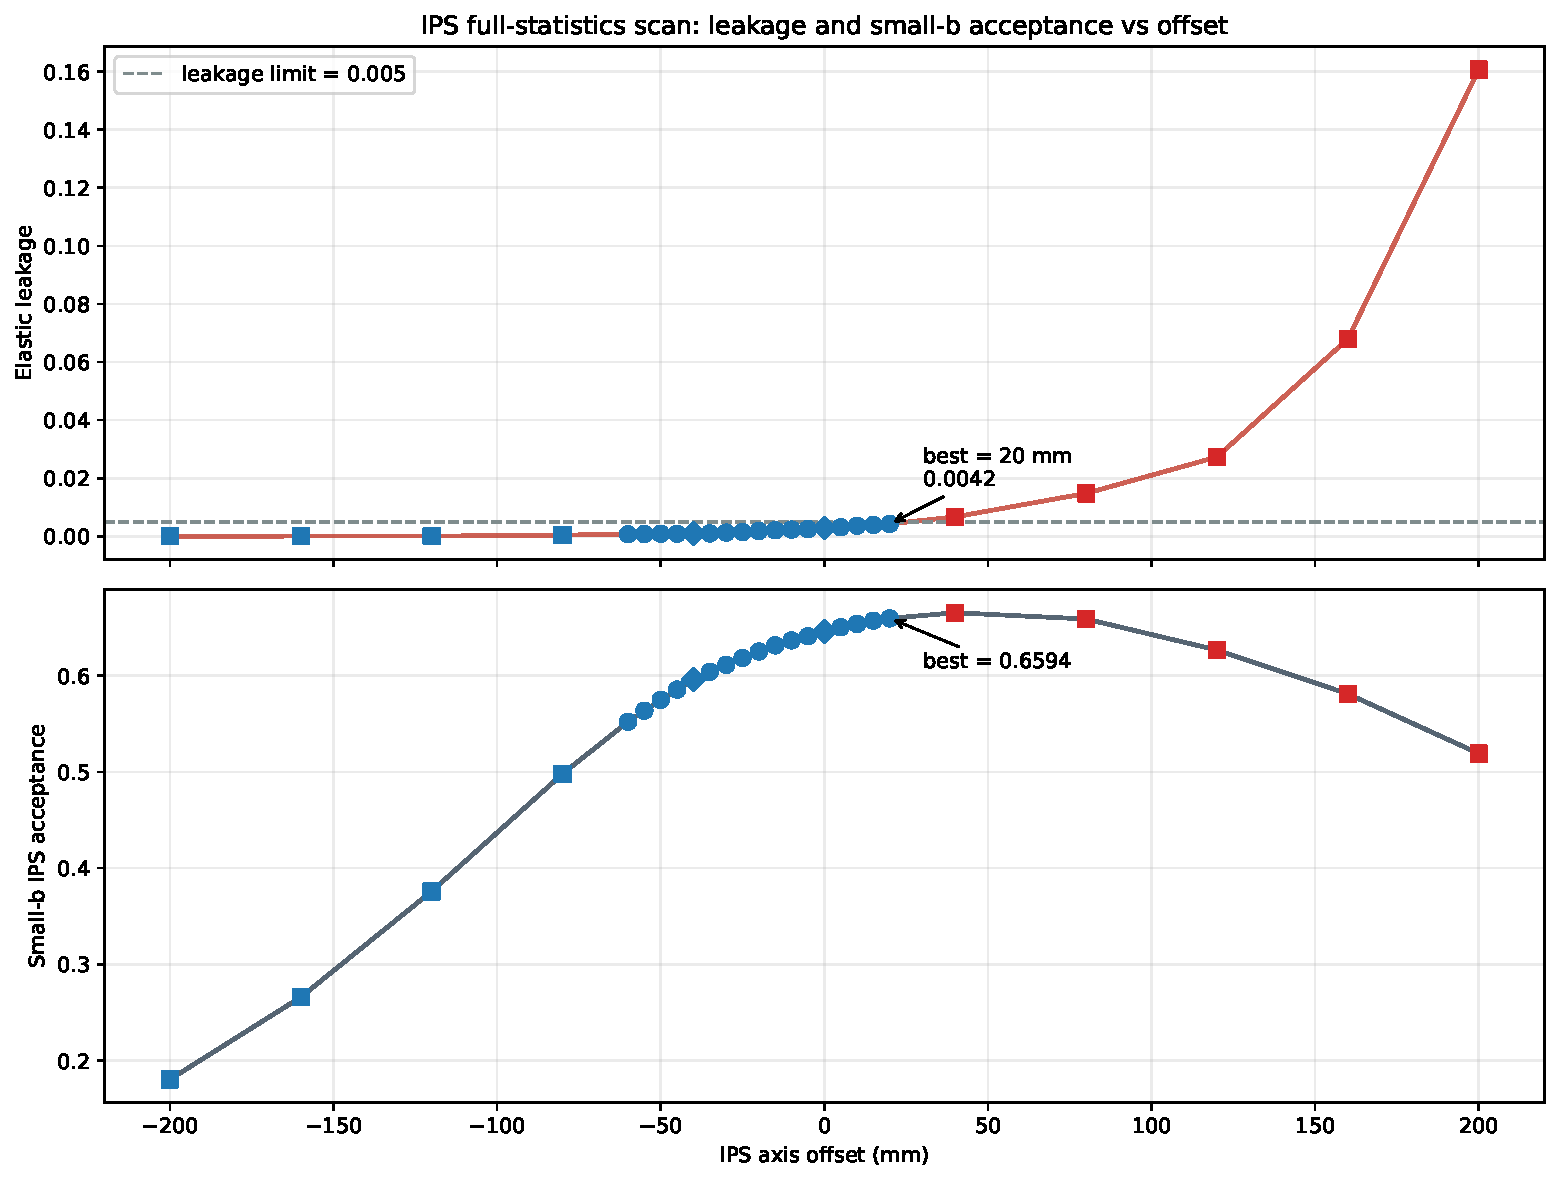
\includegraphics[width=0.6\textwidth]{assets/ips_scan_3deg_1p15T_fullstats/ips_scan_fullstats_metrics_vs_offset.pdf}
\end{frame}

\begin{frame}{Full-Statistics Result: Trade-off Curve}
\centering
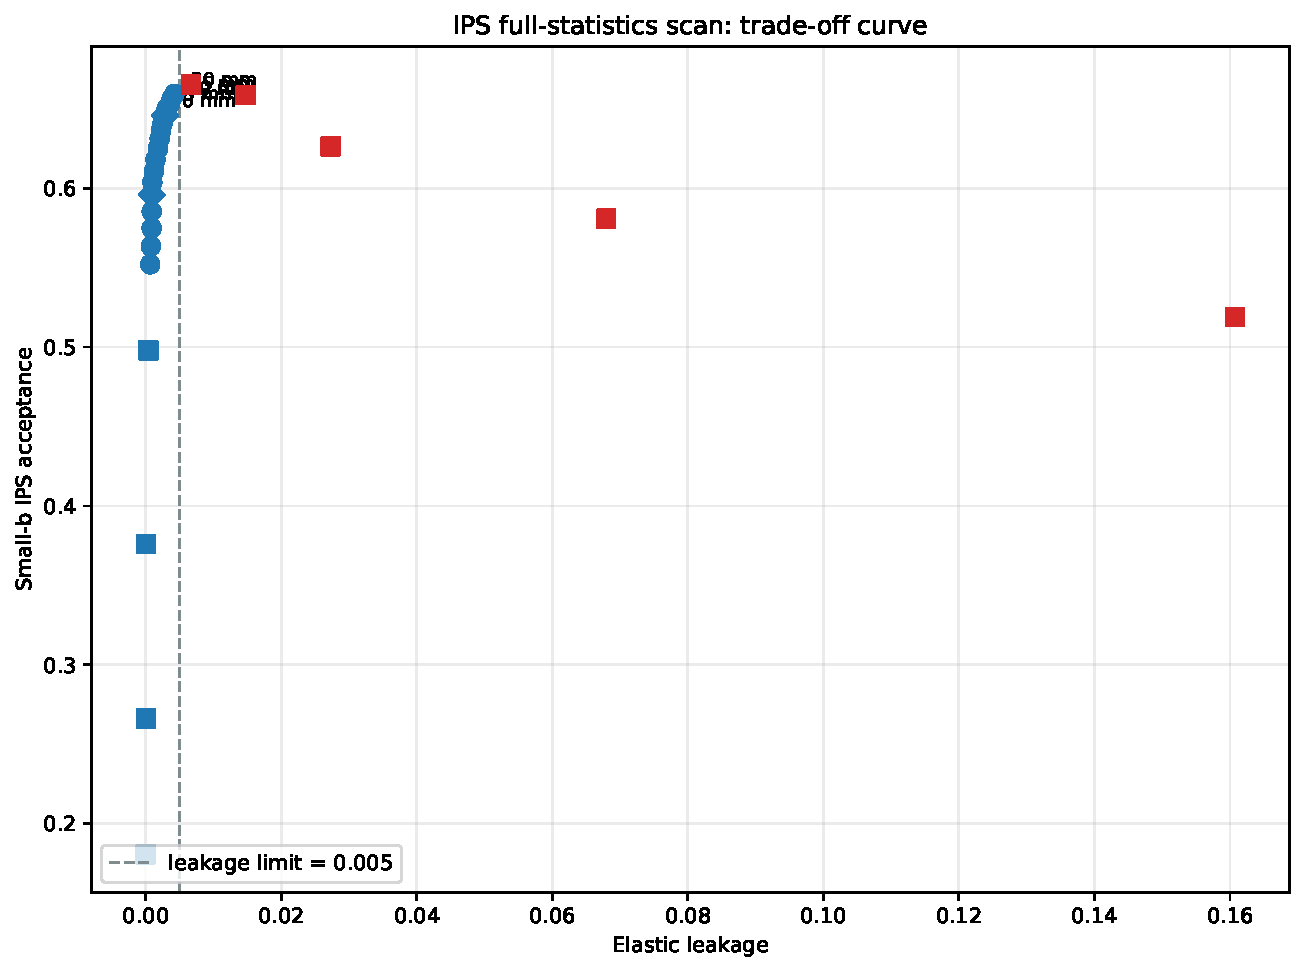
\includegraphics[width=0.68\textwidth]{assets/ips_scan_3deg_1p15T_fullstats/ips_scan_fullstats_tradeoff.pdf}
\end{frame}

\begin{frame}{Best Candidates}
\begin{table}
\centering
\small
\begin{tabular}{ccccc}
\toprule
Rank & Offset (mm) & Feasible & Elastic leakage & Small-$b$ acceptance \\
\midrule
1 & 20  & yes & 0.004248 & 0.659436 \\
2 & 15  & yes & 0.003885 & 0.656993 \\
3 & 10  & yes & 0.003626 & 0.653664 \\
4 & 5   & yes & 0.003108 & 0.650193 \\
5 & 0   & yes & 0.002849 & 0.645771 \\
\bottomrule
\end{tabular}
\end{table}

\begin{itemize}
  \item The official full-statistics recommendation is \textbf{+20 mm}.
  \item Positive offsets above 40 mm become infeasible because elastic leakage exceeds the 0.5\% requirement.
  \item The previous sampled \texttt{beamOn300} run favored \texttt{-40 mm}; the full-statistics run resolves this finite-statistics bias.
\end{itemize}
\end{frame}

\begin{frame}{Interpretation}
\begin{itemize}
  \item Moving IPS from 0 mm to +20 mm improves small-$b$ acceptance from:
  \[
    0.645771 \rightarrow 0.659436
  \]
  while still satisfying the leakage constraint.
  \item The gain is modest but systematic across the final refined positive offsets.
  \item Large positive shifts increase the overlap with elastic background too quickly.
  \item Large negative shifts remain very clean, but lose deep-inelastic coverage.
\end{itemize}
\end{frame}

\begin{frame}{Artifacts and Reproducibility}
\small
\textbf{Result directory}
\begin{itemize}
  \item \texttt{data/simulation/ips\_scan/.../smallb\_all\_noForward\_fullstats}
\end{itemize}

\textbf{Main outputs inside the result directory}
\begin{itemize}
  \item \texttt{best\_ips\_positions.txt}
  \item \texttt{ips\_scan\_summary.csv}
  \item \texttt{scan\_progress.log}
\end{itemize}

\textbf{Driver script}
\begin{itemize}
  \item \texttt{run\_ips\_position\_scan\_3deg115T\_smallb\_all\_noforward\_fullstats.sh}
\end{itemize}

\textbf{Plotting script}
\begin{itemize}
  \item \texttt{scripts/analysis/plot\_ips\_scan\_metrics.py}
\end{itemize}
\end{frame}

\begin{frame}{Take-away}
\begin{block}{Recommendation}
For the current Geant4 configuration (\texttt{3deg\_1.15T}, target-reference-only, no-forward, full statistics), the preferred IPS position is:
\[
  \boxed{\text{\texttt{AxisOffset = +20 mm}}}
\]
\end{block}

\begin{itemize}
  \item Elastic leakage: 0.4248\%.
  \item Small-$b$ acceptance: 65.94\%.
  \item This is the result to use as the current reference for further veto studies and geometry exports.
\end{itemize}
\end{frame}

\end{document}
